\documentclass[11pt,a4paper]{article}

\usepackage[T1]{fontenc}
\usepackage[utf8]{inputenc}
\usepackage{lmodern}
\usepackage[a4paper,margin=0.86in,headheight=22pt]{geometry}
\usepackage{amsmath,amssymb,booktabs,graphicx,tabularx,array}
\usepackage{microtype}
\usepackage{xcolor}
\usepackage{titlesec}
\usepackage{caption}
\usepackage{enumitem}
\usepackage[round,authoryear]{natbib}
\usepackage{fancyhdr}
\usepackage{tocloft}
\usepackage[hidelinks]{hyperref}
\usepackage{bookmark}
\usepackage{xurl}

\definecolor{ink}{HTML}{1F2933}
\definecolor{accent}{HTML}{2458A6}
\definecolor{accentlight}{HTML}{EDF3FC}
\definecolor{muted}{HTML}{52606D}

\hypersetup{
  colorlinks=true,
  linkcolor=accent,
  citecolor=accent,
  urlcolor=accent,
  pdftitle={When Communication Amplifies Error},
  pdfauthor={Veronika Loran}
}

\setlength{\parindent}{0pt}
\setlength{\parskip}{0.55em}
\setlength{\emergencystretch}{2em}
\setlist{nosep,leftmargin=*}
\renewcommand{\arraystretch}{1.18}
\setcounter{tocdepth}{2}
\renewcommand{\contentsname}{Contents}
\renewcommand{\cftsecfont}{\bfseries\color{accent}}
\renewcommand{\cftsecpagefont}{\bfseries\color{accent}}
\renewcommand{\cftsecleader}{\cftdotfill{\cftdotsep}}
\setlength{\cftbeforesecskip}{0.65em}
\setlength{\cftbeforesubsecskip}{0.15em}

\titleformat{\section}{\large\bfseries\color{accent}}{\thesection}{0.65em}{}
\titleformat{\subsection}{\normalsize\bfseries\color{ink}}{\thesubsection}{0.55em}{}
\titlespacing*{\section}{0pt}{1.4em}{0.45em}
\titlespacing*{\subsection}{0pt}{1.0em}{0.25em}

\captionsetup{font=small,labelfont={bf,color=accent},textfont=it,justification=raggedright,singlelinecheck=false}

\pagestyle{fancy}
\fancyhf{}
\fancyhead[L]{\footnotesize\scshape Communication, correlation, and collective failure}
\fancyhead[R]{\footnotesize Veronika Loran}
\fancyfoot[C]{\footnotesize\color{muted}\thepage}
\renewcommand{\headrulewidth}{0.35pt}
\renewcommand{\headrule}{\hbox to\headwidth{\color{accent}\leaders\hrule height \headrulewidth\hfill}}

\title{\textbf{When Communication Amplifies Error:}\\[0.25em]
\large Correlated Collective Failure in Networked Binary Agents}
\author{Veronika Loran}
\date{15 September 2026}

\begin{document}

% --------------------------------------------------------------------------
% Cover sheet and contents
% --------------------------------------------------------------------------
\hypersetup{pageanchor=false}
\begin{titlepage}
\thispagestyle{empty}
{\color{accent}\rule{\textwidth}{2pt}}
\vspace{0.6cm}
{\small\bfseries\color{accent}\MakeUppercase{Computational research / Preprint}}\par
\vspace{1.3cm}
{\fontsize{34}{39}\selectfont\bfseries\color{ink} When Communication\\ Amplifies Error\par}
\vspace{0.7cm}
{\LARGE\color{accent} Correlated Collective Failure\\ in Networked Binary Agents\par}
\vspace{0.7cm}
{\large\color{muted} A controlled study of shared information,\\ social influence, and collective reliability\par}
\vfill
\begingroup
\setlength{\fboxsep}{16pt}
\colorbox{accentlight}{\begin{minipage}{\dimexpr\textwidth-32pt\relax}
{\small\bfseries\color{accent} THE CENTRAL QUESTION}\par\medskip
{\Large\color{ink} Can a group agree almost completely\\ and still be wrong?\par}\medskip
{\normalsize\color{muted} Communication can combine independent evidence. It can also amplify a shared mistake. This paper measures both outcomes in a controlled model.}
\end{minipage}}
\endgroup
\vfill
{\Large\bfseries\color{ink} Veronika Loran}\par
\vspace{0.3cm}
{\small\color{muted} Results-aware preprint, version 1.1\quad /\quad 15 September 2026}\par
\vspace{0.7cm}
{\small\itshape\color{muted} The evidence supports a finite-horizon communication--correlation mechanism. A thermodynamic phase transition is not claimed.}\par
\vspace{0.5cm}
{\color{accent}\rule{\textwidth}{2pt}}
\end{titlepage}

\clearpage
\pagenumbering{roman}
\hypersetup{pageanchor=true}
\begingroup
\fontsize{9.5}{11.5}\selectfont
\setlength{\parskip}{0pt}
\setlength{\cftbeforesecskip}{0.35em}
\setlength{\cftbeforesubsecskip}{0pt}
\tableofcontents
\endgroup
\clearpage
\pagenumbering{arabic}
\setcounter{page}{1}

% --------------------------------------------------------------------------
% Main manuscript
% --------------------------------------------------------------------------
\begin{abstract}
Communication is often introduced to help a population pool distributed evidence. It can also cause agents to reuse the same evidence and thereby convert a shared input error into a collective failure. This paper studies that trade-off in a stochastic binary-agent model with sparse communication, controlled private-signal quality, and crossed shared-input correlation. In the reduced confirmation experiment at $N=256$, $T=200$, $q=0.55$, and $\rho_{\mathrm{in}}=0.25$, strong communication ($J=3$) produced near-consensus (agreement $=0.994$) but low mean individual accuracy ($=0.401$) and high severe-failure risk ($=0.60$). The matched independent-input condition reached accuracy $=0.946$ with severe-failure risk $=0.05$. In a separate, lower-replication terminal-error experiment, strong coupling reduced the effective population size to approximately one, indicating that additional agents contributed little independent error cancellation at the terminal time. A smaller-population replication and a four-family topology screen preserved the broad contrast, although the replication did not reproduce a negative paired accuracy change in every cell. Approximate-equilibrium checks on a complete graph showed increasing ordering in a coupling window containing the analytic mean-field scale but did not resolve finite-size scaling. The results therefore support a finite-horizon communication--correlation mechanism and motivate stronger population-size and mixing studies; they do not establish a thermodynamic phase transition.
\end{abstract}

\vspace{0.25em}
\noindent\textbf{Keywords:} collective intelligence; social influence; correlated errors; networked agents; heat-bath dynamics; finite-size scaling; collective risk

\section{Introduction}

\subsection{Motivation}

The central promise of a group is that it can combine partial and noisy information. If different members make sufficiently diverse errors, aggregation can outperform the typical member and sometimes the best individual. This is the intuition behind the wisdom-of-crowds literature, but the independence condition is fragile. Once people or agents observe one another, their decisions become statistically dependent. Agreement can then increase even when the information available to the group has not improved.

The distinction between agreement and correctness is particularly important in systems that make repeated decisions under communication. An agent that sees a neighbor's decision does not necessarily receive a new measurement of the underlying state. It may instead receive a transformed copy of an already-counted signal. Repeatedly copying that signal can suppress the independent variation that makes majority aggregation effective. If the copied signal is wrong, social coupling may therefore create a population that is highly coherent and systematically mistaken.

This paper examines that possibility using a binary reference model. The model is intentionally simple enough to support exact checks and transparent causal contrasts. It includes a hidden binary truth, noisy private signals, a tunable common information source, a graph of social interactions, and asynchronous stochastic updates. The resulting system can be studied both as a finite-horizon decision process and, for symmetric interactions, as a Markov chain with a known stationary distribution. Keeping these two interpretations separate is essential: a finite-time cascade is not automatically an equilibrium phase transition.

\subsection{Related work}

The theoretical starting point is the study of social averaging and opinion convergence. DeGroot's consensus model formalized repeated weighted averaging, while the Friedkin--Johnsen model added persistent individual anchors \citep{degroot1974,friedkin_johnsen1990}. These models clarify how network influence determines convergence, but they do not by themselves distinguish a consensus that is accurate from one that is merely stable.

Work on collective estimation has shown both beneficial and harmful effects of social information. Golub and Jackson linked learning quality to the concentration of influence in social networks \citep{golub_jackson2010}. Becker, Brackbill, and Centola demonstrated that network structure can shape the way social information improves collective estimation \citep{becker2017}. Jayles and colleagues showed that the quality and quantity of social information matter for collective estimation performance \citep{jayles2017}. In contrast, Lorenz and colleagues showed that social influence can reduce diversity without producing a corresponding accuracy gain \citep{lorenz2011}. Our study takes the tension between these findings as a design requirement: useful aggregation and harmful dependence must be measured in the same experiment.

Informational cascades provide a complementary mechanism. In the model of Bikhchandani, Hirshleifer, and Welch, later decisions can rationally follow earlier actions even when private information points elsewhere \citep{bikhchandani1992}. The present model is not a sequential rational-learning model, but it shares the structural feature that social information can be reused as if it were independent evidence. The explicit shared-input control allows us to separate the effect of marginal signal quality from the effect of common error.

The connection to artificial multi-agent systems is now direct. Recent work reports conviction and consensus regimes in interacting language-model communities \citep{physics_of_agents_2026}; that study fits a statistical-mechanics description to observed LLM communities, whereas the present work uses a reference model with known truth and independently controlled signal dependence. The Interaction Tax study reports that exchanging complete solutions can erase diversity under matched resource budgets \citep{interaction_tax_2026}; the present model does not claim to match token or compute budgets and exchanges binary decisions instead. Multi-agent debate provides a contrasting example in which structured interaction can improve reasoning and factuality \citep{du_et_al_2023}. These studies motivate the application context, but they do not replace a controlled stochastic baseline in which signal quality, signal dependence, communication strength, time horizon, and population size are separately specified.

\subsection{Research questions and hypotheses}

The paper addresses three questions:

\begin{enumerate}
  \item \textbf{Performance:} When does communication improve individual and collective decisions relative to an otherwise matched uncoupled population?
  \item \textbf{Mechanism:} Does shared input interact with communication by increasing terminal error covariance and reducing the effective number of independent decision-makers?
  \item \textbf{Critical behavior:} Are observed changes compatible with a thermodynamic phase transition, or are they better described as finite-time crossovers, ordering, or metastable outcomes?
\end{enumerate}

These questions give rise to the following pre-specified hypotheses and interpretive rules:

\begin{itemize}
  \item \textbf{H1 (benefit):} At some tested communication strengths, mean individual accuracy increases relative to $J=0$ when private signals are sufficiently diverse.
  \item \textbf{H2 (failure):} Communication increases severe collective-failure probability under at least one shared-input condition.
  \item \textbf{H3 (dependence):} The failure-prone condition exhibits higher terminal error covariance and a smaller effective population size.
  \item \textbf{H4 (finite-size caution):} The executed size and time sweeps are not sufficient to establish a positive asymptotic failure probability or a thermodynamic transition.
  \item \textbf{H5 (robustness):} The communication--correlation interaction persists in a limited screen of sparse graph families, without implying topology invariance.
\end{itemize}

\subsection{Contribution and scope}

The contribution is a controlled mechanism account with four features. First, the construction holds marginal private-signal quality fixed while varying common-source correlation. Second, it reports accuracy, majority performance, agreement, and severe-failure risk separately. Third, it measures dependence directly from terminal error vectors rather than inferring it from visual consensus. Fourth, it treats finite-horizon decisions and equilibrium diagnostics as different objects. The study does not claim novelty for consensus dynamics, Ising-like models, the generic observation that communication can help or hurt, or a measured phase transition in the application model.

\section{Model and theoretical reference points}

\subsection{Population, truth, and graph}

There are $N$ agents indexed by $i=1,\ldots,N$. A hidden truth $Y\in\{-1,+1\}$ is sampled uniformly. Agent $i$ receives a private signal $S_i\in\{-1,+1\}$ and maintains a public binary decision $a_i(t)\in\{-1,+1\}$. The population is connected by an undirected graph $G$ with adjacency matrix $A$ and normalized interaction matrix $W$. The main reference ensemble is a connected random 8-regular graph with
\[
W_{ij}=A_{ij}/8,
\]
so that every agent receives a social field that is an average of eight neighbors. The graph is redrawn across graph replications, while the same graph is reused across paired communication conditions.

The graph is not intended to be a realistic model of a particular institution or software architecture. It is a controlled sparse interaction ensemble with fixed degree and a symmetric normalization. This choice permits a clean comparison between communication strength and information dependence; topology is examined separately in the robustness screen.

\subsection{Private signals and controlled input correlation}

Every private signal has the same marginal quality,
\[
\Pr(S_i=Y)=q,
\]
but signals need not be independent. To generate dependence, the simulation draws a common signal $Z$ with quality $q$, independent private signals $U_i$ with quality $q$, and independent copy indicators
\[
B_i\sim\operatorname{Bernoulli}(p),\qquad p=\sqrt{\rho_{\mathrm{in}}}.
\]
It then sets $S_i=Z$ when $B_i=1$ and $S_i=U_i$ otherwise. The construction preserves the marginal signal quality while varying the probability that two agents use the same latent source.

Let $X_i=\mathbf{1}\{S_i=Y\}$. Conditional on $Y$, $\operatorname{Var}(X_i)=q(1-q)$. Since two agents both copy the common signal with probability $p^2$, and otherwise their correctness indicators are conditionally independent,
\begin{equation}
\operatorname{Cov}(X_i,X_j\mid Y)=p^2q(1-q)=\rho_{\mathrm{in}}q(1-q),
\end{equation}
which gives $\operatorname{Corr}(X_i,X_j\mid Y)=\rho_{\mathrm{in}}$ for $0<q<1$. The two principal input conditions are therefore $\rho_{\mathrm{in}}=0$ (independent sources) and $\rho_{\mathrm{in}}=0.25$ (shared-source dependence), with $q\in\{0.55,0.65\}$ in the main confirmation.

\subsection{Asynchronous heat-bath dynamics}

Agents update asynchronously. At each event, an agent $i$ is selected uniformly and resampled according to
\begin{equation}
\Pr\!\left(a_i\leftarrow+1\mid a_{-i},S,G\right)=
\sigma\!\left(2\left[H S_i+J\sum_jW_{ij}a_j\right]\right),
\qquad \sigma(x)=\frac{1}{1+e^{-x}}.
\label{eq:update}
\end{equation}
Here $H$ is the weight of private evidence and $J\ge0$ is the social-coupling strength. Unless otherwise stated, $H=0.5$. One sweep consists of $N$ update events, so the finite-horizon endpoint $T$ is measured in sweeps. The default initialization is natural initialization: each agent's initial decision is drawn from the private-signal field with probability $\sigma(2HS_i)$. Separate robustness runs use other initializations where specified.

The update is stochastic even when all agents have identical signals. This is useful for two reasons. It prevents deterministic tie-breaking from creating artificial order, and it makes the difference between social alignment and truth alignment observable in repeated episodes. The simulation never gives the dynamics access to $Y$ except through the signals; truth is used only after the terminal state to score performance.

\subsection{Stationary distribution and the equilibrium distinction}

For symmetric $W$, the update rule satisfies detailed balance with respect to
\begin{equation}
\pi(a\mid S,G)=\frac{1}{\mathcal{Z}(S,G)}\exp\!\left(H\sum_iS_i a_i+\frac{J}{2}\sum_{ij}W_{ij}a_i a_j\right),
\label{eq:stationary}
\end{equation}
where $\mathcal{Z}(S,G)$ is the partition function. Exact enumeration for small systems and implementation checks give a maximum detailed-balance residual of $1.8\times10^{-18}$. Equation~\ref{eq:stationary} establishes what equilibrium would mean for a fixed signal realization and graph; it does not imply that a run observed after $T=50$ or $T=200$ sweeps has mixed.

For the complete graph at zero private field, the large-$N$ mean-field equation is
\[
m=\tanh(Jm).
\]
The nonzero solution first appears at $J_c=1$. This analytic scale is used as a code and interpretation benchmark. The application model differs from this benchmark because it has a private field, truth-aligned signal disorder, sparse graphs, finite horizons, and shared-input mixtures.

\subsection{Information-theoretic baselines}

At $J=0$, the natural initialization gives each agent an independent stochastic decision conditional on its private signal. The expected individual accuracy has the closed form
\begin{equation}
A_{\mathrm{ind}}(J=0)=
(1-q)+(2q-1)\sigma(2H).
\label{eq:j0baseline}
\end{equation}
For $H=0.5$, this predicts approximately $0.523$ at $q=0.55$ and $0.569$ at $q=0.65$, providing a baseline check on the simulated uncoupled rows.

The raw-signal majority is Bayes optimal when signals are conditionally independent and the prior over $Y$ is uniform. Under the shared-source construction, the correct Bayes oracle must marginalize over the latent common signal. Let $p=\sqrt{\rho_{\mathrm{in}}}$ and define
\[
\ell(s_i\mid y,z)=(1-p)\Pr(U_i=s_i\mid y)+p\mathbf{1}\{s_i=z\}.
\]
Then the posterior is proportional to
\begin{equation}
\Pr(Y=y\mid s)\propto \frac{1}{2}\sum_{z\in\{-1,+1\}}
\Pr(Z=z\mid y)\prod_{i=1}^{N}\ell(s_i\mid y,z).
\label{eq:oracle}
\end{equation}
This oracle is evaluated from the observed signals and is not supplied to the agents. It is an information-theoretic benchmark for expected zero-one accuracy under the specified signal model, not a deterministic ceiling for every finite sample and not a ceiling on the stochastic heat-bath dynamics' agreement.

\section{Experimental design}

\subsection{Overview of executed batches}

The evidence package contains exploratory, confirmatory, mechanistic, robustness, size/time, and equilibrium components. Their roles and limitations are kept separate in Table~\ref{tab:design}. The main confirmation was intentionally smaller than the planned allocation; this is a scope limitation, not a hidden change to the endpoint.

\begin{table}[htbp]
\centering
\caption{Executed batches and their interpretive roles. A graph--signal instance is the primary replication unit for the finite-horizon studies.}
\label{tab:design}
\small
\begin{tabularx}{\textwidth}{@{}l l c c X@{}}
\toprule
Batch & Role & $N$ & $T$ & Allocation and interpretation \\
\midrule
Pilot & Exploration & 128 & 100 & 48 cells; 16 trajectories per cell; reduced exploratory map. \\
Confirmation & Primary contrast & 256 & 200 & 4 graphs $\times$ 5 signals; 20 graph--signal instances per cell. \\
Replication & Scale check & 128 & 100 & 10 graphs $\times$ 10 signals; 100 instances per cell at $J\in\{0,3\}$. \\
Mechanism & Error dependence & 128 & 100 & 40 instances per cell with retained terminal error vectors. \\
Size/time & Boundary diagnostic & 32$-$256 & 50, 200 & 1 graph $\times$ 5 signals; descriptive only. \\
Topology & Robustness screen & 128 & 100 & 4 sparse families; 25 instances per family and cell. \\
Equilibrium & Criticality benchmark & 16$-$64 & -- & Complete graph, $H=0$; 10 chains, burn-in and thinning. \\
Provenance protocol & Exploratory alternative & 128 & 100 & 10 graphs $\times$ 10 signals; one-pass private-signal comparator; not used for primary inference. \\
\bottomrule
\end{tabularx}
\end{table}

\subsection{Confirmation and replication allocation}

The reduced confirmation varied $J\in\{0,1.5,3,4\}$, $q\in\{0.55,0.65\}$, and $\rho_{\mathrm{in}}\in\{0,0.25\}$ at $N=256$ and $T=200$. Each cell contained four graph instances and five signal realizations per graph. The contrast of $J=3$ against $J=0$ was the central strong-coupling comparison; $J=1.5$ and $J=4$ show whether the result is restricted to a single value.

The replication used fresh seeds and increased replication to 100 graph--signal instances per cell, but changed the population size to $N=128$ and the horizon to $T=100$. It therefore tests whether the direction of the interaction survives a scale and time change; it is not a claim of exact duplication. The mechanism batch was run separately because terminal error vectors were not stored in the earlier confirmation file.

A separate exploratory protocol audit used the same $N=128$, $T=100$, $q=0.55$, and $\rho_{\mathrm{in}}=0.25$ slice with 10 graphs and 10 signal instances per protocol. It compared the repeated-decision heat-bath dynamics with a one-pass protocol in which each agent receives a weighted average of neighbors' private signals once. This comparator is labelled \texttt{source\_tagged\_one\_pass} in the execution files, but it does not deduplicate agents that happen to share the latent common source and it changes the information representation. It is therefore treated as exploratory protocol evidence, not as a validated provenance intervention or as part of the primary confirmatory family.

\subsection{Pairing and randomization}

The main treatment contrasts reuse the same graph, truth, signal realization, initialization stream, update-index stream, and heat-bath uniforms across $J$ values whenever mathematically valid. The varied coupling $J$ is excluded from the treatment random stream. This design turns much of the comparison into a paired contrast and reduces noise from unrelated graph and signal draws.

Graph, truth, shared-source, private-signal, copy-indicator, initialization, update-index, and heat-bath streams are derived from stable hashed namespaces. The raw rows retain configuration hashes, graph and signal identifiers, trajectory identifiers, pair identifiers, seeds or seed namespaces, and terminal error vectors in the later batches. Failed or incomplete jobs are not silently converted into successful rows.

\subsection{Estimands and metrics}

For a terminal state, define the loss, magnetization, and truth-aligned magnetization as
\[
L=\frac{1}{N}\sum_i\mathbf{1}(a_i\ne Y),\qquad
m=\frac{1}{N}\sum_i a_i,\qquad
r=Ym.
\]
The reported metrics are:

\begin{itemize}
  \item \textbf{Individual accuracy:} $A_{\mathrm{ind}}=1-L$, averaged over terminal episodes.
  \item \textbf{Majority accuracy:} one if $r>0$, zero if $r<0$, and one half if $r=0$.
  \item \textbf{Agreement:} $|m|$, which is high for both all-correct and all-wrong consensus.
  \item \textbf{Severe failure:} the indicator $\mathbf{1}(L\ge0.9)$, implemented as at least $\lceil0.9N\rceil$ wrong agents.
  \item \textbf{Information ceilings:} raw-signal majority and the latent-source Bayes oracle, both scored against the same truth.
\end{itemize}

The primary estimands are the paired changes
\[
\Delta A_{\mathrm{ind}}=E[A_{\mathrm{ind}}(J)-A_{\mathrm{ind}}(0)],
\qquad
\Delta R=E[R(J)-R(0)],
\]
where $R$ denotes the severe-failure indicator and the expectation is over the declared graph--signal replication design. No claim is made that three tested coupling values define a continuous beneficial or failure region.

\subsection{Error covariance and effective population size}

For terminal error vectors $e_i=\mathbf{1}(a_i\ne Y)$, let $p_i=E[e_i]$ and define the average marginal variance
\[
\bar v=\frac{1}{N}\sum_i p_i(1-p_i).
\]
Across repeated episodes, the variance of the population loss contains both marginal error variance and cross-agent covariance. The average pair covariance is reconstructed as
\begin{equation}
\bar C=\frac{N\operatorname{Var}(L)-\bar v}{N-1},
\qquad
\rho_{\mathrm{eff}}=\frac{\bar C}{\bar v},
\qquad
N_{\mathrm{eff}}=\frac{\bar v}{\operatorname{Var}(L)}.
\label{eq:neff}
\end{equation}
If errors are independent and homogeneous, $N_{\mathrm{eff}}$ is close to $N$. If errors are shared, the population can have a much smaller effective size even when its physical size is large. The reported quantities are aggregate, finite-sample diagnostics. Heterogeneity and sampling noise can make $\rho_{\mathrm{eff}}$ slightly exceed one.

\subsection{Uncertainty and inference policy}

Point estimates are means over terminal episodes. The result files include ordinary bootstrap intervals for the compact summaries. Later replication and topology analyses additionally use a hierarchical bootstrap: graph instances are resampled at the outer level and signal instances are resampled within graph. This avoids treating multiple signals from the same graph as fully independent graph replications.

The study emphasizes effect sizes and uncertainty ranges rather than a single omnibus significance test. For the primary confirmation, the ordinary bootstrap summaries in \path{results/confirmation_summary.csv} resample the 20 terminal graph--signal rows within each cell. Table~\ref{tab:primaryuncertainty} additionally reports 95\% two-level bootstrap intervals for the paired effects, resampling the four graph clusters and then signal instances within each selected graph; the calculation uses 20,000 replicates and is stored in \path{analysis/confirmation/primary_uncertainty.csv}. Because only four graph clusters were available, these intervals are descriptive and can be broad; they do not substitute for a larger confirmatory sample. The size/time sweep has five signal instances per cell, and the critical benchmarks have limited mixing resolution. The analysis therefore reports null, adverse, and supportive cells rather than selecting only favorable outcomes.

\subsection{Implementation validation}

The implementation was checked with nine automated tests. These cover graph normalization and degree constraints, the signal marginal and correlation formulas, exact transition and detailed-balance calculations, the complete-graph mean-field coupling, global sign symmetry, Bayes-oracle enumeration for small systems, metric edge cases, covariance identities, and agreement between optimized and reference update calculations. The theory diagnostic reports $J_c=1$ at zero private field and a detailed-balance residual below $2\times10^{-18}$.

\section{Results}

\subsection{Central confirmation contrast}

Table~\ref{tab:mainresults} reports the $J=0$ and $J=3$ endpoints for both signal qualities and both input-correlation conditions. At $q=0.55$ with independent inputs, the strong-coupling condition improved individual accuracy from $0.528$ to $0.946$ and increased agreement from $0.068$ to $0.993$. Majority accuracy was high in both cases, increasing from $0.85$ to $0.95$.

At the same marginal signal quality with $\rho_{\mathrm{in}}=0.25$, communication produced nearly identical agreement ($0.994$) but reduced individual accuracy from $0.493$ to $0.401$ and raised severe-failure probability from zero observed episodes to $0.60$. This is the key separation in the paper: the population became more aligned while becoming less correct. The latent-source Bayes oracle scored $0.90$ in this cell, showing that the observed signal vector contains recoverable information under the specified model; the failure is therefore not forced by an information-theoretic ceiling at accuracy $0.40$.

The paired point estimates are large but should be read with the available replication in view. For the central $q=0.55$ contrast, $\Delta A_{\mathrm{ind}}=+0.418$ with independent inputs and $-0.092$ with shared inputs; the corresponding changes in severe-failure risk are $+0.05$ and $+0.60$. The cluster-aware intervals in Table~\ref{tab:primaryuncertainty} are broad because the confirmation contains only four graph clusters. In particular, they support a strong finite-sample contrast while leaving the population-level magnitude uncertain.

\begin{table}[htbp]
\centering
\caption{Reduced confirmation endpoints for the weak and strong coupling conditions. Estimates are means over 20 graph--signal instances per cell at $N=256$ and $T=200$; paired uncertainty intervals for the primary $J=3$ effects are reported in Table~\ref{tab:primaryuncertainty}.}
\label{tab:mainresults}
\small
\begin{tabular}{@{}llcrrrr@{}}
\toprule
Inputs & $q$ & $J$ & $A_{\mathrm{ind}}$ & Majority & Agreement & Severe failure \\
\midrule
Independent ($\rho_{\mathrm{in}}=0$) & 0.55 & 0 & 0.528 & 0.85 & 0.068 & 0.00 \\
Independent ($\rho_{\mathrm{in}}=0$) & 0.55 & 3 & 0.946 & 0.95 & 0.993 & 0.05 \\
Shared ($\rho_{\mathrm{in}}=0.25$) & 0.55 & 0 & 0.493 & 0.40 & 0.227 & 0.00 \\
Shared ($\rho_{\mathrm{in}}=0.25$) & 0.55 & 3 & 0.401 & 0.40 & 0.994 & 0.60 \\
Independent ($\rho_{\mathrm{in}}=0$) & 0.65 & 0 & 0.569 & 1.00 & 0.139 & 0.00 \\
Independent ($\rho_{\mathrm{in}}=0$) & 0.65 & 3 & 0.946 & 0.95 & 0.990 & 0.05 \\
Shared ($\rho_{\mathrm{in}}=0.25$) & 0.65 & 0 & 0.581 & 0.70 & 0.250 & 0.00 \\
Shared ($\rho_{\mathrm{in}}=0.25$) & 0.65 & 3 & 0.699 & 0.70 & 0.995 & 0.30 \\
\bottomrule
\end{tabular}
\end{table}

\begin{table}[htbp]
\centering
\caption{Paired primary effects and descriptive 95\% two-level bootstrap intervals. Each estimate compares $J=3$ with $J=0$ at $N=256$ and $T=200$; intervals resample four graph clusters and signal instances nested within each selected graph.}
\label{tab:primaryuncertainty}
\small
\begin{tabularx}{\textwidth}{@{}X c X X c@{}}
\toprule
Inputs & $q$ & $\Delta A_{\mathrm{ind}}$ & $\Delta$ severe failure & Units \\
\midrule
Independent ($\rho_{\mathrm{in}}=0$) & 0.55 & $+0.418\;[+0.192,+0.498]$ & $+0.05\;[0.00,0.25]$ & 20 \\
Shared ($\rho_{\mathrm{in}}=0.25$) & 0.55 & $-0.092\;[-0.408,+0.350]$ & $+0.60\;[0.00,1.00]$ & 20 \\
Independent ($\rho_{\mathrm{in}}=0$) & 0.65 & $+0.377\;[+0.165,+0.446]$ & $+0.05\;[0.00,0.25]$ & 20 \\
Shared ($\rho_{\mathrm{in}}=0.25$) & 0.65 & $+0.118\;[-0.243,+0.367]$ & $+0.30\;[0.00,0.75]$ & 20 \\
\bottomrule
\end{tabularx}
\end{table}

The $q=0.65$ rows show that higher marginal quality reduces but does not eliminate the dependence problem. Under independent inputs, $J=3$ again produced accuracy near $0.946$ and severe-failure risk of $0.05$. Under shared inputs, accuracy rose relative to the $J=0$ baseline but remained far below the independent-input condition, while severe-failure risk reached $0.30$. This is consistent with a mechanism in which communication can exploit diverse information but cannot reliably distinguish a common error from a trustworthy consensus.

\begin{figure}[htbp]
\centering
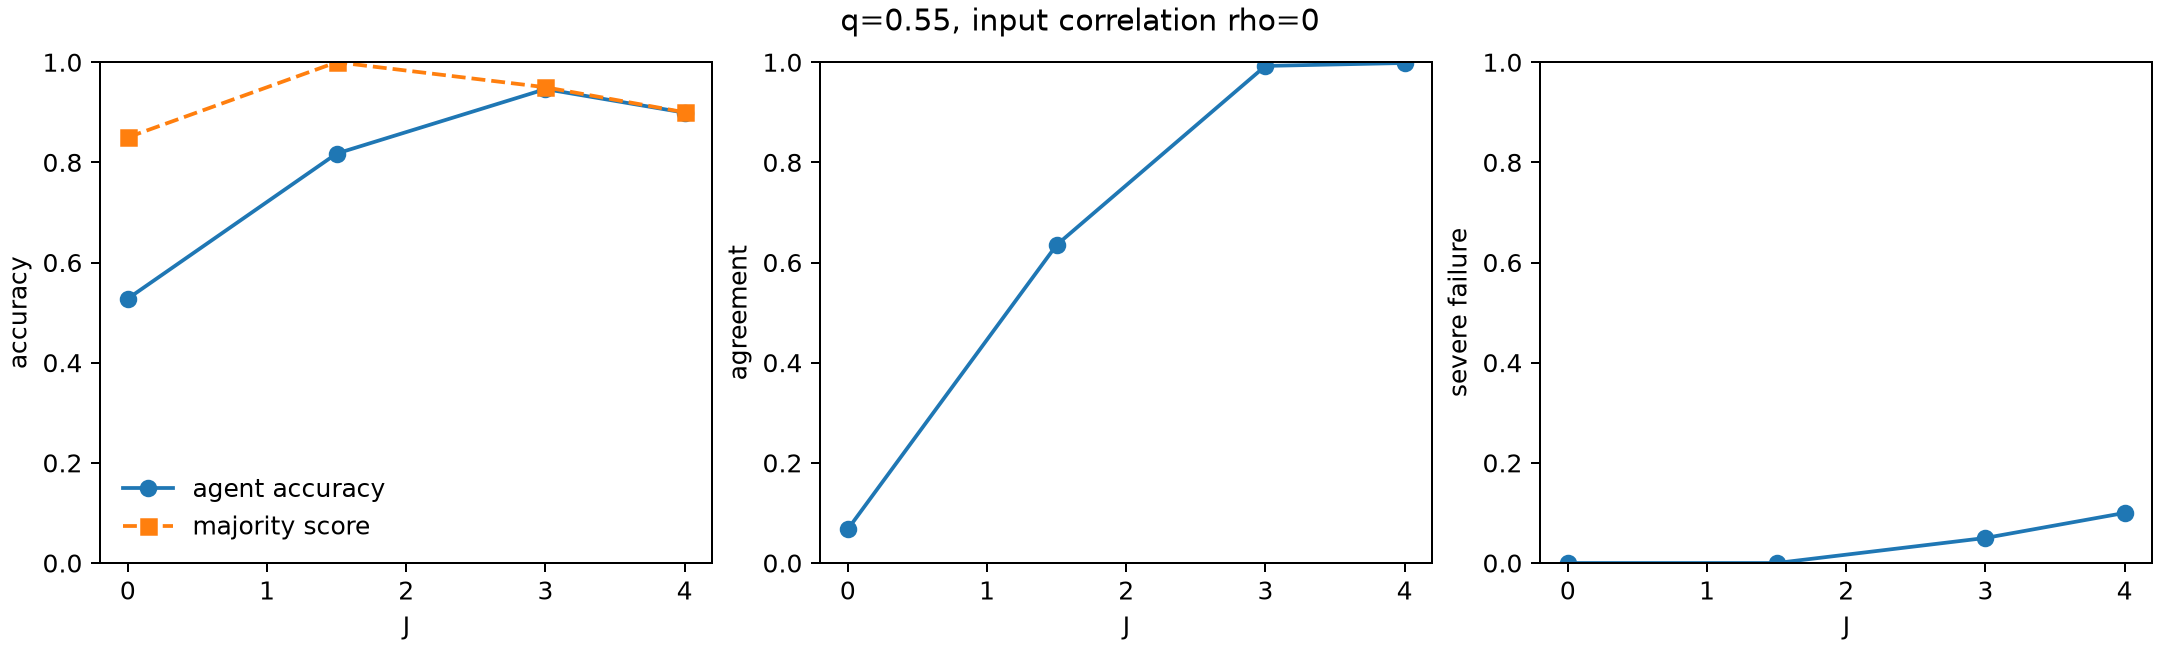
\includegraphics[width=0.96\linewidth]{../results/figures/confirmation/confirmation_q0.55_rho0.png}
\caption{Reduced confirmation curves for independent inputs at $q=0.55$. Accuracy, majority performance, and agreement are shown as functions of the coupling strength; severe failure remains low in the tested range.}
\label{fig:independent}
\end{figure}

\begin{figure}[htbp]
\centering
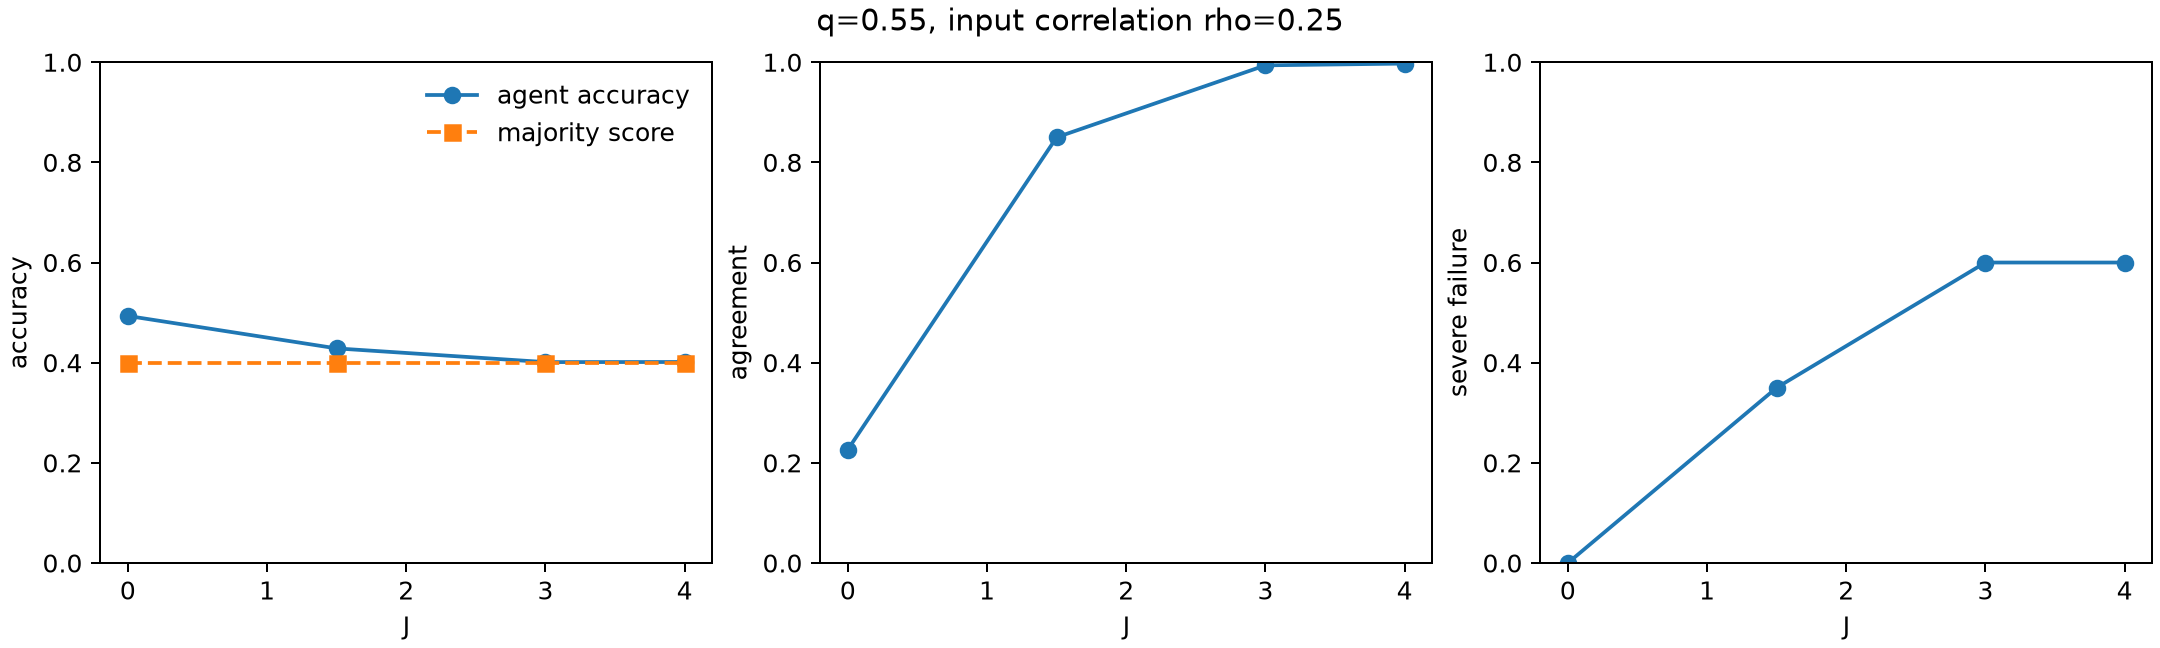
\includegraphics[width=0.96\linewidth]{../results/figures/confirmation/confirmation_q0.55_rho0.25.png}
\caption{Reduced confirmation curves for shared inputs at $q=0.55$. Agreement approaches one while individual accuracy remains below one half and severe-failure risk rises.}
\label{fig:correlated}
\end{figure}

\subsection{Coupling range and paired effect sizes}

The central contrast is not limited to one plotted endpoint. At $q=0.55$ and $\rho_{\mathrm{in}}=0.25$, the $J=1.5$ confirmation condition had accuracy $0.429$, agreement $0.850$, and severe-failure risk $0.35$, while $J=4$ had accuracy $0.401$, agreement $0.997$, and risk $0.60$. The strong-coupling adverse outcome therefore emerges before the final tested value and persists at the upper edge.

For independent inputs at $q=0.55$, the corresponding $J=1.5$, $J=3$, and $J=4$ accuracies were $0.818$, $0.946$, and $0.899$. The non-monotonicity at $J=4$ is a reminder that strong communication is not synonymous with optimal communication. Agreement continued to increase, but individual accuracy did not improve monotonically. At $q=0.65$ and independent inputs, accuracy increased from $0.569$ at $J=0$ to $0.889$ at $J=1.5$ and $0.946$ at $J=3$, with a small decline to $0.899$ at $J=4$.

The paired contrast ledger reports mean changes from $J=0$. At $q=0.55$, $J=3$ increased accuracy by $0.418$ under independent inputs but decreased it by $0.092$ under shared inputs. The severe-failure change was $0.05$ and $0.60$, respectively. At $q=0.65$, the corresponding accuracy changes were $0.377$ and $0.118$, while severe-failure changes were $0.05$ and $0.30$. These point estimates are consistent with H1 and H2 at the tested anchors, but their cluster-aware intervals remain wide; they do not establish a general phase boundary or a precisely estimated population effect.

\subsection{Replication and sparse topology robustness}

The fresh $N=128$, $T=100$ replication increases graph--signal replication to 100 units per cell. At $q=0.55$, $J=3$ yielded accuracy $0.747$ and severe-failure risk $0.25$ with independent inputs, compared with accuracy $0.609$ and risk $0.39$ with shared inputs. At $q=0.65$, the corresponding accuracies were $0.938$ and $0.620$, with severe-failure risks $0.06$ and $0.38$. The absolute effects are less extreme than in the $N=256$, $T=200$ confirmation. The shared-input arm still has lower accuracy and higher severe-failure risk than the independent-input arm at $J=3$, but the replication does not reproduce a negative paired accuracy change in the shared $q=0.55$ cell ($\Delta A_{\mathrm{ind}}=+0.070$). It therefore supports the broader dependence contrast while qualifying the stronger claim that communication must reduce mean accuracy in every finite-horizon replication.

The topology screen compares random-regular, Watts--Strogatz, two-block stochastic block, and preferential-attachment graphs at $N=128$ and $T=100$. It uses 25 graph--signal instances per family and cell. In the low-quality shared-input condition at $J=3$, severe-failure estimates were $0.44$ for all four families, while agreement ranged from $0.963$ to $0.994$. Under independent inputs, severe-failure estimates ranged from $0.24$ to $0.36 and agreement from $0.831$ to $0.993. The shared-input failure mechanism therefore survives the tested topology changes, although the screen is too small to support topology invariance or asymptotic robustness.

\begin{table}[htbp]
\centering
\caption{Replication and topology-screen summaries at $J=3$ and $N=128$. Topology entries are ranges across the four sparse graph families.}
\label{tab:robustness}
\small
\begin{tabular}{@{}llrrrr@{}}
\toprule
Source & Condition & $q$ & Accuracy & Agreement & Severe failure \\
\midrule
Replication & $\rho_{\mathrm{in}}=0$ & 0.55 & 0.747 & 0.992 & 0.25 \\
Replication & $\rho_{\mathrm{in}}=0.25$ & 0.55 & 0.609 & 0.995 & 0.39 \\
Replication & $\rho_{\mathrm{in}}=0$ & 0.65 & 0.938 & 0.995 & 0.06 \\
Replication & $\rho_{\mathrm{in}}=0.25$ & 0.65 & 0.620 & 0.996 & 0.38 \\
Topology range & $\rho_{\mathrm{in}}=0$ & 0.55 & 0.637$-$0.751 & 0.831$-$0.993 & 0.24$-$0.36 \\
Topology range & $\rho_{\mathrm{in}}=0.25$ & 0.55 & 0.558$-$0.561 & 0.963$-$0.994 & 0.44 \\
Topology range & $\rho_{\mathrm{in}}=0$ & 0.65 & 0.864$-$0.964 & 0.939$-$0.954 & 0.00$-$0.12 \\
Topology range & $\rho_{\mathrm{in}}=0.25$ & 0.65 & 0.598$-$0.640 & 0.971$-$0.996 & 0.36$-$0.40 \\
\bottomrule
\end{tabular}
\end{table}

Because the implemented symmetric normalization divides by the graph's mean degree, and the preferential-attachment family is degree-heterogeneous, this is a robustness screen across graph ensembles rather than a topology-only intervention.

\subsection{Error covariance and effective population size}

The mechanism batch retained terminal error vectors so that agreement could be connected to dependence directly. At $q=0.55$ and $\rho_{\mathrm{in}}=0.25$, the uncoupled condition had $\rho_{\mathrm{eff}}=0.049$ and $N_{\mathrm{eff}}=17.6$ over 40 episodes. At $J=1.5$, these values changed to $0.731$ and $1.36$. At $J=3$, they were $1.016$ and $0.984$; at $J=4$, they were $1.026$ and $0.975$.

The interpretation is not that an individual simulation literally contains one agent. Rather, the terminal loss behaves as though it were generated by roughly one effective error draw because the agents' errors move together. The effect is also visible in the higher-replication $N=128$ run: in the shared-input cell, $N_{\mathrm{eff}}$ was approximately $1.00$ at $J=3$ and $17.9$ at $J=0$. The corresponding effective correlation was approximately one at $J=3$ and $0.048$ at $J=0$.

These covariance quantities are nonlinear, aggregate diagnostics estimated from 40 or 100 terminal error vectors; uncertainty intervals for $N_{\mathrm{eff}}$ are not reported because the small-sample ratio can be unstable. The primary confirmation does not contain error vectors, so the covariance evidence is independent supporting evidence rather than a post hoc reanalysis of the main endpoint.

\begin{table}[htbp]
\centering
\caption{Terminal error-dependence diagnostics for the low-quality shared-input condition. Values are aggregate summaries reconstructed from retained error vectors.}
\label{tab:covariance}
\small
\begin{tabular}{@{}llrrrr@{}}
\toprule
Batch & $J$ & $\rho_{\mathrm{in}}$ & $\rho_{\mathrm{eff}}$ & $N_{\mathrm{eff}}$ & Episodes \\
\midrule
Mechanism & 0 & 0.25 & 0.049 & 17.61 & 40 \\
Mechanism & 1.5 & 0.25 & 0.731 & 1.36 & 40 \\
Mechanism & 3 & 0.25 & 1.016 & 0.984 & 40 \\
Mechanism & 4 & 0.25 & 1.026 & 0.975 & 40 \\
Replication & 0 & 0.25 & 0.048 & 17.92 & 100 \\
Replication & 3 & 0.25 & 1.001 & 0.999 & 100 \\
\bottomrule
\end{tabular}
\end{table}

\subsection{Exploratory one-pass protocol audit}

The additional protocol audit provides a useful but non-confirmatory diagnostic of feedback. In the correlated low-quality slice at $N=128$ and $T=100$, the repeated-decision heat-bath protocol at $J=3$ reached accuracy $0.600$, agreement $0.995$, and severe-failure risk $0.40$. The one-pass private-signal comparator reached accuracy $0.608$, agreement $0.802$, and risk $0.10$ over the same number of graph--signal units. The lower agreement and tail risk are compatible with less repeated decision feedback, but they cannot be attributed to provenance alone: the comparator changes the message representation and does not deduplicate agents that share the latent source. We therefore treat this result as a diagnostic that motivates a properly controlled provenance experiment, not as evidence for a validated intervention.

\subsection{Population size and decision horizon}

The reduced size/time sweep changes $N$ and $T$ at a correlated low-quality slice. At $J=3$, $q=0.55$, and $\rho_{\mathrm{in}}=0.25$, agreement was close to one in every tested cell, but accuracy and severe-failure risk varied by population size. Severe-failure rates at $T=50$ were $0.60$, $0.20$, $0.40$, and $0.20$ for $N=32,64,128,256$; the corresponding $T=200$ rates were the same. Accuracy ranged from $0.394$ to $0.799$ across these cells.

The near equality between the two horizons does not prove horizon independence. The sweep uses only one graph and five signal instances per cell, so the latent shared-source mixture dominates the uncertainty. It shows that the failure-prone regime is not confined to a single population size, but it cannot distinguish a decreasing asymptotic risk from a positive floor, nor can it establish an order-of-limits result.

\begin{figure}[htbp]
\centering
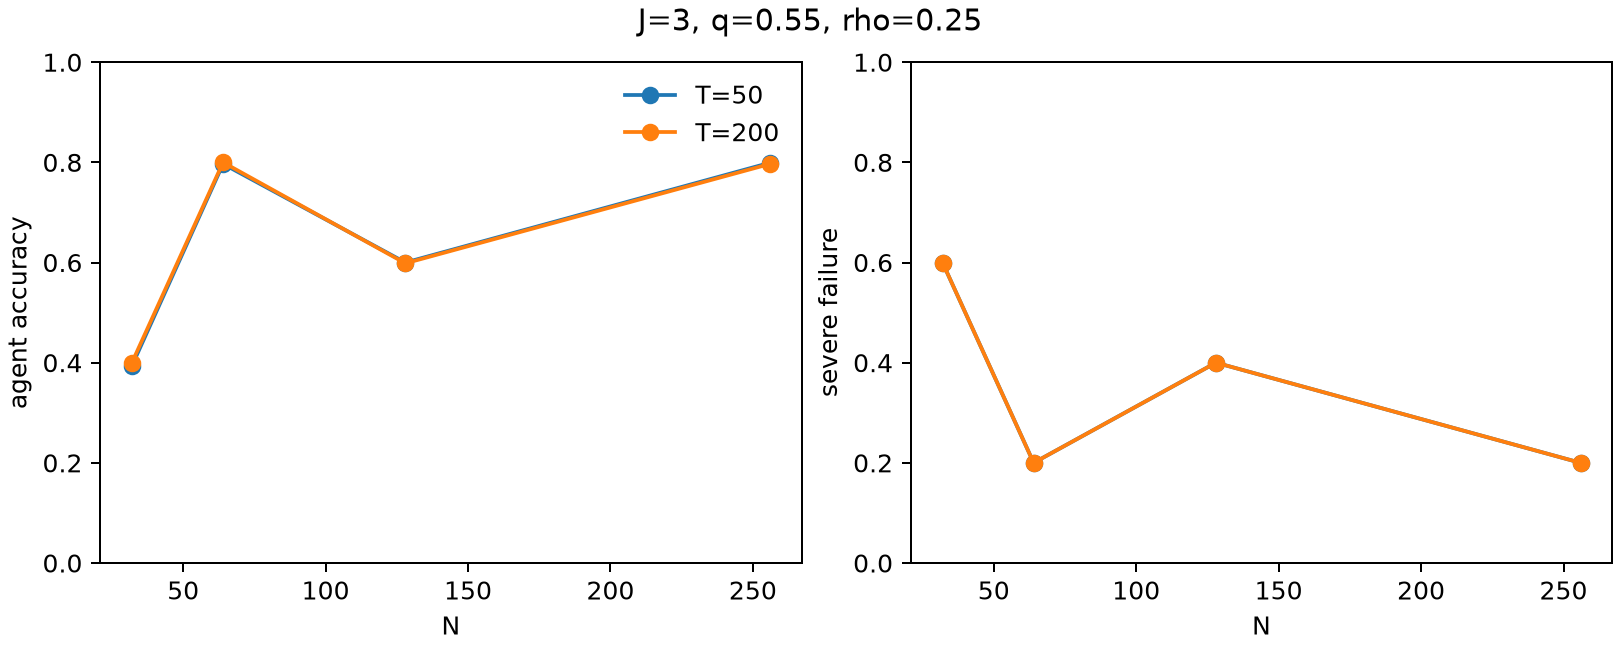
\includegraphics[width=0.96\linewidth]{../results/figures/scaling/scaling_q0.55_rho0.25_J3.png}
\caption{Reduced size/time sweep for the correlated low-quality slice at $J=3$. The same qualitative near-consensus pattern coexists with substantial variation in accuracy and severe-failure risk across the small, sparsely replicated size range.}
\label{fig:scalingcorrelated}
\end{figure}

\begin{figure}[htbp]
\centering
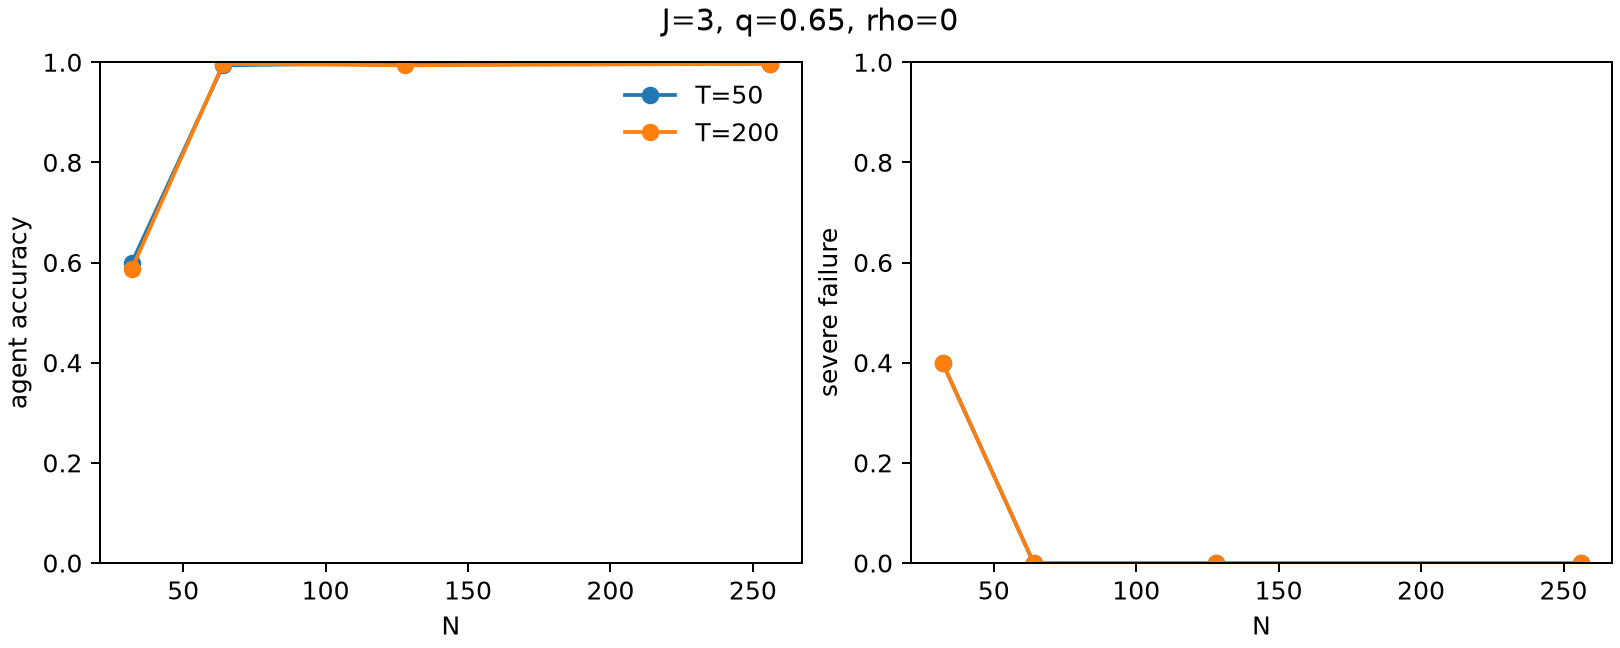
\includegraphics[width=0.96\linewidth]{../results/figures/scaling/scaling_q0.65_rho0_J3.png}
\caption{Reduced size/time sweep for the independent higher-quality slice at $J=3$. Strong coupling produces high accuracy and low severe-failure risk in this tested regime.}
\label{fig:scalingindependent}
\end{figure}

\begin{table}[htbp]
\centering
\caption{Size/time sweep at $J=3$, $q=0.55$, and $\rho_{\mathrm{in}}=0.25$. One graph and five signal instances were used per cell.}
\label{tab:scaling}
\small
\begin{tabular}{@{}rrr rr r@{}}
\toprule
$N$ & $T$ & Accuracy & Agreement & Severe failure & Majority \\
\midrule
32 & 50 & 0.394 & 0.988 & 0.60 & 0.40 \\
32 & 200 & 0.400 & 1.000 & 0.60 & 0.40 \\
64 & 50 & 0.797 & 0.994 & 0.20 & 0.80 \\
64 & 200 & 0.800 & 1.000 & 0.20 & 0.80 \\
128 & 50 & 0.600 & 1.000 & 0.40 & 0.60 \\
128 & 200 & 0.598 & 0.997 & 0.40 & 0.60 \\
256 & 50 & 0.799 & 0.995 & 0.20 & 0.80 \\
256 & 200 & 0.797 & 0.994 & 0.20 & 0.80 \\
\bottomrule
\end{tabular}
\end{table}

\subsection{Equilibrium criticality benchmark}

The equilibrium analysis is deliberately separated from the application claim. For the complete graph with $H=0$ and $q=0.5$, the large-$N$ mean-field reference predicts $J_c=1$. The approximate-equilibrium run used $N\in\{16,32,64\}$, $J\in\{0.8,0.9,1.0,1.1,1.2\}$, 200 burn-in sweeps, 20 retained samples per chain, thinning by ten sweeps, and ten independent chains per condition.

Susceptibility increased with $J$ and attained its maximum at the upper tested edge $J=1.2$ for all three sizes. At this edge, the susceptibility values were $7.72$, $12.30$, and $24.74$ for $N=16,32,64$. Binder values were $0.533$, $0.526$, and $0.569$, respectively. These numbers show increasing ordering in a window that contains the analytic scale, but they do not demonstrate recovery of $J_c$; the limited size range, coupling window, chain length, and sampling resolution do not provide a resolved common crossing.

The separate finite-horizon benchmark used $N\in\{16,32,64,128\}$, ten trajectories per cell, $T=200$, and a wider coupling interval ending at $J=1.3$. Its susceptibility maximum also occurred at the upper tested boundary. Following standard finite-size diagnostics \citep{binder1981,hong2007}, the two benchmarks are treated as implementation and scale checks rather than as evidence of a measured critical exponent. The nonzero private field in the application model can round or shift symmetry-breaking behavior, and shared-input disorder introduces a different source of population-level variability.

\begin{table}[htbp]
\centering
\caption{Approximate-equilibrium complete-graph benchmark at $H=0$ and $q=0.5$. The maximum within the tested window occurs at $J=1.2$ for every size.}
\label{tab:critical}
\small
\begin{tabular}{@{}rrrrl@{}}
\toprule
$N$ & $J_{\mathrm{max}}$ & Susceptibility & Binder & Interpretation \\
\midrule
16 & 1.2 & 7.72 & 0.533 & Upper-edge maximum \\
32 & 1.2 & 12.30 & 0.526 & Upper-edge maximum \\
64 & 1.2 & 24.74 & 0.569 & Upper-edge maximum \\
\bottomrule
\end{tabular}
\end{table}

\section{Robustness, alternative interpretations, and falsification tests}

\subsection{Why agreement alone is insufficient}

The most visually striking result is the rise of agreement toward one. If agreement were used as the sole endpoint, both the independent-input benefit and the shared-input failure would look like successful coordination. The truth-aligned magnetization, individual accuracy, majority score, and severe-failure indicator show that the two trajectories are different. This is not a cosmetic distinction. In the shared-input condition, the population's consensus direction is often inherited from a common source and then reinforced by the network.

\subsection{Why the result is not simply lower signal quality}

The shared-input and independent-input arms have the same marginal $q$. Their difference is the dependence structure. The Bayes oracle explicitly conditions on the observed signals and the correct latent-source model, scoring $0.90$ in the central correlated cell. The failure therefore lies in the interaction between information dependence and repeated social updating, not in a lower marginal accuracy or an impossible inference problem.

\subsection{Why the covariance result is mechanistic evidence}

Consensus is compatible with several mechanisms, including genuine evidence accumulation, a strong truth-aligned field, or copied error. Error covariance distinguishes these possibilities. The effective population size falls from roughly 18 to roughly one in the correlated mechanism batch as $J$ increases from zero to three. The independent-input condition can also become highly correlated under strong coupling, but its errors are more often aligned with a correct aggregate because its inputs are more diverse. The mechanism is therefore the joint change in information dependence and social coupling, not communication alone.

\subsection{Alternative explanations and tests}

Several alternative explanations remain possible and are partly addressed by the execution package:

\begin{itemize}
  \item \textbf{Initialization:} Natural initialization may favor the private signal, while random or dispersed starts can alter finite-time ordering. The current primary claim is restricted to the declared initialization and horizon.
  \item \textbf{Mixing:} A short chain can appear ordered because it has not explored the stationary distribution. The equilibrium benchmark is reported separately and remains small.
  \item \textbf{Graph structure:} A random regular graph is only one sparse ensemble. The topology screen shows persistence across four families at one size but cannot test all degree, modularity, or directedness effects.
  \item \textbf{Information representation:} The exploratory one-pass comparator reduces repeated decision feedback, but it also changes the messages from public decisions to private signals and does not deduplicate latent sources. Its result cannot isolate provenance without a matched source-aware design.
  \item \textbf{Threshold choice:} Severe failure is prespecified as $L\ge0.9$. Other tail thresholds could produce different risk curves, so the reported value is an operational definition rather than a universal boundary.
  \item \textbf{Finite-sample covariance:} The covariance summaries use retained error vectors from separate batches and are not available in the original confirmation rows. This is why covariance is used as supporting mechanism evidence rather than as a post hoc replacement endpoint.
\end{itemize}

These limitations are falsifiable. Longer equilibrated chains, graph replication across six or more population sizes, alternative initializations, source-tagged communication, calibrated evidence weights, and synchronous-update comparisons could all weaken or refine the current interpretation. In particular, a failure probability that declines systematically under a prespecified increasing-$N$ and increasing-$T$ schedule would contradict an asymptotic risk-floor interpretation.

\section{Discussion}

\subsection{Principal finding}

Within the specified model and tested cells, communication has two qualitatively different operational effects. When private inputs are conditionally independent, social coupling can help the population exploit distributed evidence: individual accuracy rises, majority performance is high, and agreement increases. When the inputs share a latent error source, the same coupling can create near-consensus around an incorrect direction. The paired nature of the design, the matched marginal signal quality, the Bayes benchmark, and the error-vector diagnostics support this interpretation, while the cluster-aware intervals show that the present confirmation does not precisely estimate its population magnitude.

The result is best understood as a communication-induced dependence mechanism. The network does not manufacture a new observation. It changes how often a decision is reused, how quickly it spreads, and how much independent variation remains at the terminal time. In that sense, the effective population size is a useful bridge between collective-intelligence language and statistical-mechanics language: physical population size is not the same as the number of independent error draws.

\subsection{Relation to collective intelligence}

The findings reconcile apparently conflicting claims that communication can help and communication can hurt. Both can be true because the sign of the effect depends on the covariance structure of the information being exchanged. A network can improve a group when it directs attention toward complementary or informative evidence. It can harm the same group when it turns one erroneous source into the dominant attractor. This is consistent with the broader literature's emphasis on diversity, influence concentration, and the quality of social information \citep{lorenz2011,golub_jackson2010,becker2017,jayles2017}.

\subsection{Relation to phase-transition language}

The paper uses phase-transition concepts as a diagnostic framework, not as a label for every sharp finite-sample change. A thermodynamic claim would require a declared order of limits, equilibrated sampling, multiple population sizes, a coupling window that contains the relevant peak or crossing, and uncertainty that supports scaling rather than visual separation. The current application has none of these requirements at sufficient resolution. The complete-graph benchmark is consistent with increasing ordering in a window around the analytic mean-field scale and the approximate-equilibrium run improves the finite-horizon comparison, but neither establishes a transition in the random-field networked application.

This distinction matters for multi-agent AI research. A sharp change in consensus after a fixed number of interaction rounds could reflect a dynamical threshold, a metastable cascade, an initialization effect, or a genuine equilibrium singularity. These mechanisms have different implications for intervention and system design. Calling them all phase transitions would make the empirical conclusion less precise, not more significant.

\subsection{Practical implications}

Three design recommendations follow directly from the model:

\begin{enumerate}
  \item Measure dependence between information sources. Marginal accuracy alone does not reveal whether ten agents provide ten pieces of evidence or one copied error.
  \item Preserve provenance where possible. A system should distinguish a new observation from a repeated report of an old observation and should not count repeated copies as independent support.
  \item Display agreement beside correctness and tail risk. Optimizing consensus without an accuracy or failure metric can move a system into the high-correlation failure regime.
\end{enumerate}

These are implications for system diagnostics, not claims that the binary model quantitatively predicts human or language-model behavior.

\section{Limitations and next tests}

The reference model is deliberately controlled and is not empirically calibrated to humans, organizations, or language models. Its private evidence is binary, its social influence is symmetric, and its communication protocol repeatedly updates decisions rather than exchanging source-tagged evidence. These choices isolate the mechanism but limit external validity.

The main confirmation contains 20 graph--signal instances per cell. The size/time sweep contains one graph and five signal instances per cell. The topology screen uses four graph families at $N=128$ and $T=100$. The equilibrium benchmark reaches only $N=64$ and uses finite burn-in, thinning, and retained-sample budgets. These are adequate for a transparent evidence package and mechanism demonstration, not for a definitive phase diagram.

The primary confirmation predates terminal error-vector storage. Consequently, covariance is estimated in the mechanism, replication, topology, and scaling batches rather than reconstructed from the original confirmation CSV. The topology screen also uses a resource-limited design and should not be read as evidence that network structure is irrelevant; its graph-family comparison is partly entangled with degree heterogeneity and the chosen normalization. The prespecified E70 interventions such as reducing common-source exposure or using genuinely deduplicated, source-tagged messages were not executed. A separate one-pass private-signal comparator was run as an exploratory protocol audit, but because it changes the information representation and does not deduplicate latent sources, it is not presented as a validated control.

The next confirmatory campaign should: (i) increase signal-instance replication at the shared-source slice; (ii) use at least six population sizes with multiple graphs per size; (iii) sample fixed-horizon and approximate-equilibrium dynamics as separate experiments; (iv) include explicit order-of-limits schedules; (v) compare random-regular, modular, and heterogeneous-degree networks under matched message budgets; and (vi) test source provenance and calibrated evidence weights. An optional language-model extension should use matched token, model, evaluator, and interaction budgets and should be reported as a separate model class.

\section{Conclusion}

This study shows how a population can become more communicatively coordinated and less collectively reliable at the same time. In a controlled networked binary-agent model, communication improves performance when private evidence is diverse but amplifies severe collective failure when inputs share errors. Terminal error covariance provides mechanism evidence: strong coupling reduces the effective population size from many independent error opportunities to approximately one at the terminal time in the tested cells.

The result is a finite-horizon mechanism finding supported by confirmation, replication, covariance, and a limited topology screen. The accompanying equilibrium benchmarks are consistent with the expected mean-field ordering scale but do not resolve the finite-size scaling needed for a thermodynamic phase-transition claim. The scientifically useful conclusion is therefore conditional and operational: communication should be evaluated together with information provenance, error dependence, accuracy, and tail risk.

\section{Data and code availability}

The execution repository contains the model code, frozen JSON configurations, raw CSV outputs, generated summaries, figures, literature evidence matrix, and protocol deviations. Principal artifacts include \path{results/confirmation.csv}, \path{results/confirmation_summary.csv}, \path{results/replication.csv}, \path{results/mechanism.csv}, \path{results/mechanism_protocol.csv}, \path{results/topology.csv}, \path{results/scaling.csv}, \path{results/critical.csv}, and \path{results/critical_equilibrium.csv}, together with the corresponding files under \path{analysis/}. The paired uncertainty table is stored in \path{analysis/confirmation/primary_uncertainty.csv}. The manuscript itself is generated from \path{paper/when-communication-amplifies-error.tex}; the PDF is the typeset deliverable.

\appendix

\section{Detailed computational protocol}

\subsection{Random-stream separation}

Each job derives stable random streams from a canonical namespace containing the batch, graph identifier, signal identifier, trajectory identifier, population size, signal quality, input-correlation condition, private-field strength, horizon, initialization, and protocol. The treatment value $J$ is excluded from the stream used for paired contrasts. This permits the same graph, signal, initialization, update-event sequence, and uniforms to be reused across coupling conditions without making unrelated jobs accidentally identical.

The graph stream generates the adjacency matrix and the graph metadata. The signal stream generates $Y$, $Z$, $U_i$, and $B_i$. The trajectory stream generates natural initialization, update indices, and heat-bath uniforms. All terminal rows retain a pair identifier and configuration hash. The later error-vector batches store terminal error indicators in compact bit-string form so that covariance can be reconstructed without a dense agent-by-agent matrix.

\subsection{Batch-specific deviations}

The exploratory pilot was reduced from the planned grid because the transparent reference Python engine was computationally expensive. The confirmation was executed as a reduced allocation with four graphs and five signal instances per graph. A later replication increased the number of graph--signal instances at $N=128$ and $T=100$, and a topology screen compared four sparse families with 25 instances per family and cell. The equilibrium benchmark was limited to $N\le64$ and ten chains per condition. These deviations are recorded in \path{protocol/deviations.csv} and \path{protocol/deviations_v2.csv}; they are part of the evidence record rather than hidden exclusions.

\subsection{Reproducibility checks}

The test suite checks the following properties: graph symmetry and normalization; signal marginal quality and conditional correlation; the $J=0$ accuracy formula; sign-reversal symmetry; Bayes-oracle agreement with small-system enumeration; exact detailed balance; stationary transition normalization; covariance reconstruction; metric behavior for ties and constant states; optimized/reference update agreement; and configuration validation. The current suite contains nine passing tests.

\section{Derivations and interpretation of diagnostic quantities}

\subsection{Signal-correlation construction}

For completeness, conditional on $Y=y$, the correctness indicator for the common signal is $C_Z=\mathbf{1}\{Z=y\}$ and the correctness indicator for an independent signal is $C_i=\mathbf{1}\{U_i=y\}$. Both are Bernoulli$(q)$. The correctness indicator for agent $i$ is $X_i=B_iC_Z+(1-B_i)C_i$. Independence of $B_i$, $B_j$, $C_Z$, $C_i$, and $C_j$ except for the shared $C_Z$ term gives
\[
E[X_i\mid Y]=q,
\qquad
E[X_iX_j\mid Y]-q^2=p^2q(1-q),
\]
which yields the correlation stated in the main text. The construction is therefore a controlled way to vary source dependence without changing the marginal signal quality.

\subsection{Uncoupled stochastic baseline}

At $J=0$, the update probability depends only on $HS_i$. If $S_i=Y$, the decision is correct with probability $\sigma(2H)$. If $S_i\ne Y$, it is correct with probability $1-\sigma(2H)$. Averaging over the signal gives equation~\ref{eq:j0baseline}. This baseline is not the raw signal accuracy $q$ because natural initialization samples a stochastic decision from the heat-bath field.

\subsection{Effective population size}

Let $L=N^{-1}\sum_i e_i$. Then
\[
\operatorname{Var}(L)=\frac{1}{N^2}\left[\sum_i\operatorname{Var}(e_i)+\sum_{i\ne j}\operatorname{Cov}(e_i,e_j)\right].
\]
Replacing the first sum by $N\bar v$ and solving for the average off-diagonal covariance gives $\bar C$ in equation~\ref{eq:neff}. The quantity $N_{\mathrm{eff}}=\bar v/\operatorname{Var}(L)$ equals $N$ under independent homogeneous errors and falls when the loss fluctuates more than independent aggregation predicts. It is an interpretable diagnostic of redundancy, not a literal population count.

\section{Interpretive guardrails}

The following rules govern the claims in this manuscript:

\begin{enumerate}
  \item Agreement is not evidence of truth. Every consensus result is reported with an accuracy or majority metric.
  \item A finite-horizon result is not labeled equilibrium unless a separate sampling protocol is used and its mixing limitations are reported.
  \item A susceptibility peak at the boundary of a tested coupling window is not a critical-point estimate.
  \item Error covariance is computed from retained terminal error vectors and is not inferred from agreement alone.
  \item Reduced replication supports a mechanism and motivates further work; it does not support a universal phase diagram.
  \item The binary-agent model is a reference system. Any human or LLM interpretation requires a separate, resource-matched validation study.
\end{enumerate}

\phantomsection
\addcontentsline{toc}{section}{References}
\bibliographystyle{plainnat}
\bibliography{references}

\end{document}
